% To compile, run PDFLaTeX, then bibtex, then PDFLaTex again


\documentclass[conference]{IEEEtran}
\IEEEoverridecommandlockouts
\usepackage{cite}
\usepackage{amsmath,amssymb,amsfonts}
\usepackage{algorithmic}
\usepackage{graphicx}
\usepackage{textcomp}
\usepackage{xcolor}
\usepackage{float}
\newcommand{\BibTeX}{\textrm{B \kern -.05em \textsc{i \kern -.025em b} \kern -.08em
T \kern -.1667em \lower .7ex \hbox{E} \kern -.125emX}}
\begin{document}


    \title{Open-Source Radiation Hardening Simulator: Design, Implementation, and Applications}

    \author{
        \IEEEauthorblockN{Jacob Anderson}
        \IEEEauthorblockA{\textit{Department of Electrical and Computer Engineering} \\
        \textit{BYU}\\
        Provo, UT, USA \\
        jacobdanderson@gmail.com}
        \and
        \IEEEauthorblockN{David Nichols}
        \IEEEauthorblockA{\textit{Department of Electrical and Computer Engineering} \\
        \textit{BYU}\\
        Provo, UT, USA \\
        dav1111@byu.edu}
        \and
        \IEEEauthorblockN{Collin Lambert}
        \IEEEauthorblockA{\textit{Department of Electrical and Computer Engineering} \\
        \textit{BYU}\\
        Provo, UT, USA \\
        collinml@byu.edu}
        \and
        \IEEEauthorblockN{Parker Allred}
        \IEEEauthorblockA{\textit{Department of Electrical and Computer Engineering} \\
        \textit{BYU}\\
        Provo, UT, USA \\
        parkerallred@email.com}
    }

    \maketitle

    \begin{abstract}
        This paper presents the design, implementation, and applications of an open-source radiation hardening simulator developed using Xschem and NGSpice.
        The simulator aims to address the challenges of simulating radiation effects on electronic circuits by providing a comprehensive library and user-friendly interface.
        The project integrates core modules for fault injection, radiation effect simulation, including Single Event Effects (SEE) and Total Ionizing Dose (TID), along with thorough documentation and examples to support users in their research and development efforts.
        Preliminary tests demonstrate the simulator's improved accuracy in modeling radiation effects, offering significant potential for future research and development.
    \end{abstract}

    \begin{IEEEkeywords}
        radiation hardening, electronic circuits, fault injection, simulation, Xschem, NGSpice
    \end{IEEEkeywords}


    \section{Introduction}\label{sec:introduction}
    The accurate simulation of radiation effects on electronic circuits is a key step in the development of robust systems in space, nuclear, and other radiation-prone environments.
    Radiation can induce a variety of faults and errors in electronic components, leading to system failures.
    Thus, understanding and mitigating these effects is essential for ensuring the reliability of electronic systems~\cite{Wrobel2011, Florian1986}.

    Natural radiation is known to be a significant source of microelectronics failure, impacting various applications from aerospace to ground-level electronics.
    To predict the reliability of these devices, tools like MC-ORACLE and RADSPICE have been developed to simulate the effects of radiation on microelectronic materials~\cite{Wrobel2011, Florian1986}.

    In this paper, we introduce an open-source radiation hardening simulator that leverages Xschem and NGSpice.
    This tool is designed to simulate and analyze the effects of radiation on electronic circuits, and aims to facilitate the development and testing of radiation-hardened designs.
    Our approach includes simulating Single Event Effects (SEE) using advanced models such as adaptive double exponential current sources and Total Ionizing Dose (TID) effects to improve the accuracy of simulations~\cite{Pepper1990}.

    The paper is structured as follows: Section II provides an overview of the project, including its background, objectives, and scope.
    Section III details the methodology and implementation, describing the integration of Xschem, NGSpice, and custom-developed modules.
    Section IV presents the testing, results, and discussion, highlighting the system's performance and the challenges encountered.
    Finally, Section V concludes the paper and outlines future work.


    \section{Project Overview}\label{sec:project-overview}
    This section provides an overview of the project, including background, objectives, and scope.

    \subsection{Background and Related Work}\label{subsec:background-and-related-work}
    Advancements in radiation hardening simulation have resulted in the development of numerous methodologies designed to enhance precision and minimize error.
    Despite these advancements, many existing techniques encounter challenges, including non-linearity, sensitivity to environmental conditions, and intricate calibration processes.
    Numerous efforts to improve these models have been undertaken, yielding significant success.
    Our open-source models are based on several of these advancements, most notably the adaptive double exponential model, which has proven effective in accurately modeling certain Single-Event Effects (SEEs)~\cite{}.

    \subsection{Project Scope and Objectives}\label{subsec:project-scope-and-objectives}
    There are multiple existing Radiation-Hardened SPICE simulatiors; however, these simulators are not open-sourced, limiting their accessibility to users who can afford to purchase these software environments.
    The primary objective of this project was to develop an open-source, radiation-effects SPICE simulator that is both user-friendly and accurate in its modeling capabilities.
    This was accomplished by researching various contemporary methods and modules for modeling radiation effects in circuits and integrating them into existing open-source SPICE programs, specifically Xschem for the front-end and NGSpice for the back-end.
    Additionally, we ensured that the interface for applying these methods was intuitive, facilitating their integration into users' projects.


    \section{Methodology and Implementation}\label{sec:methodology-and-implementation}
	A goal of this project is to present a user friendly and intutive experience to the user. To effectuate this, we've chosen to implement each radiation effect as a block that can be placed and connected to other compoenents in Xschem. A description of each block is as follows:

    \vspace{1em}

    \subsection{Single Event Effect [SEE] Simulation}\label{subsec:single-event-effect-[see]-simulation}

    \subsubsection{Double Exponential Current Source}
    A simple way to model the photo-current generated in a reverse biased pn junction due to a radiation strike, is with a double exponential current source. This method has existed for decades and has been widely used. Figure \ref{fig:double_exp} depicts a double exponential waveform.

    \begin{figure}[htbp]
        \centering
        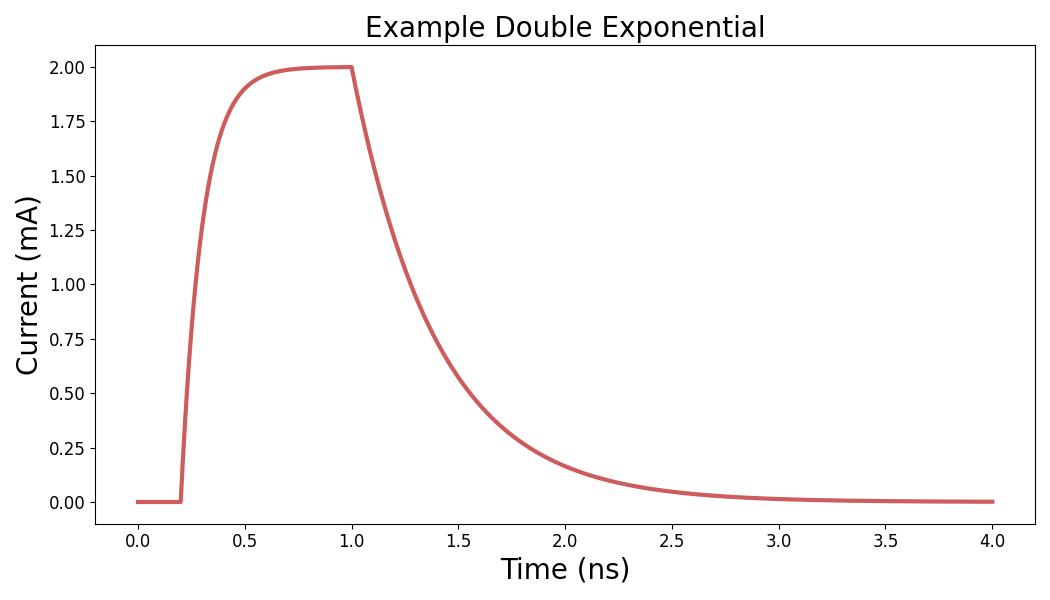
\includegraphics[width=0.95\linewidth]{EX_Double_Exponential}
        \caption{Double exponential waveform}
        \label{fig:double_exp}
    \end{figure}

    \subsubsection{Dual Double Exponential Current Source}
    A limitation of the simple double exponential current source is that it can be inaccurate in some scenarios.
    It has been found that a more realistic photo-current waveform consists of an initial peak followed by a plateau region caused by limitations of PMOS drive current in CMOS circuitry, and a final drop off.
    This waveform can be represented by adding two double exponential current sources together resulting in a dual double exponential current source. Figure \ref{fig:dual_double_exp} depicts a dual double exponential waveform. \cite{Black2015}
    \vspace{1em}

    \begin{figure}[htbp]
        \centering
        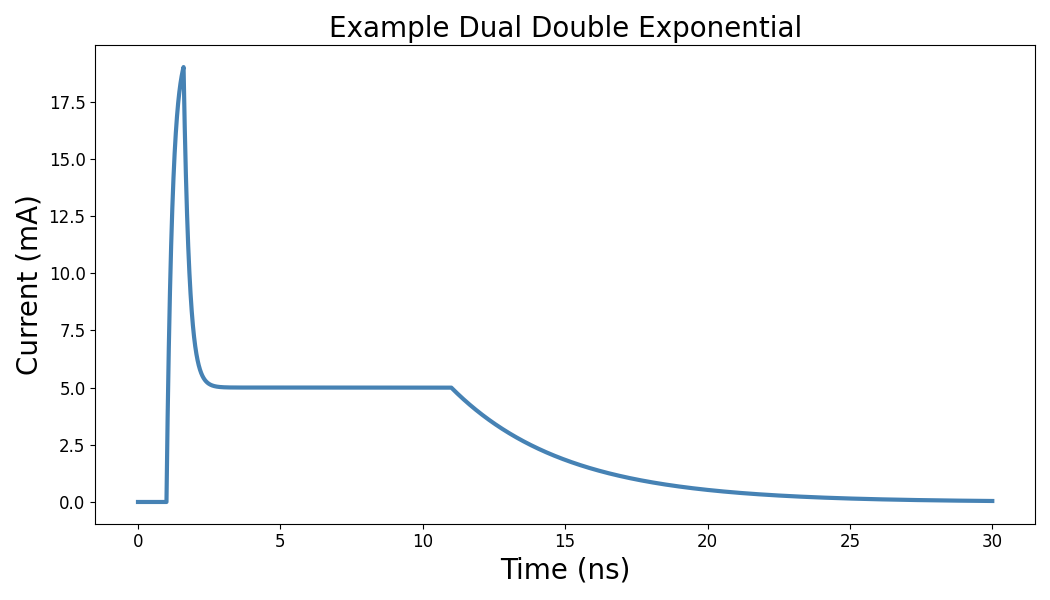
\includegraphics[width=0.95\linewidth]{EX_Dual_Double_Exponential}
        \caption{Dual double exponential waveform}
        \label{fig:dual_double_exp}
    \end{figure}

    \subsubsection{Adaptive Double Exponential Current Source}
    A problem that arises when using either the double or dual double exponential current models is that these models can produce unrealistic node voltages.
    If, for example, a double or dual double exponential current source is placed from the drain to the body node of a reverse biased NMOS transistor, when the current source is activated, the drain node voltage can be pulled below the ground node voltage.
    This means that the NMOS transistor is no longer held in reverse bias and no current should be flowing.

    The adaptive double exponential current source solves this problem by adjusting the drive current proportional to the voltage across the reverse bias PN junction of the transistor for which a radiation strike is being simulated for.
    This adjustment allows the node voltage to drop to near zero and remain at this level until the radiation induced current spike is complete.
    The resulting current waveform, as seen in figure \ref{fig:inverter_response}, closely resembles that of a dual double exponential current source.

    \begin{figure}[htbp]
        \centering
        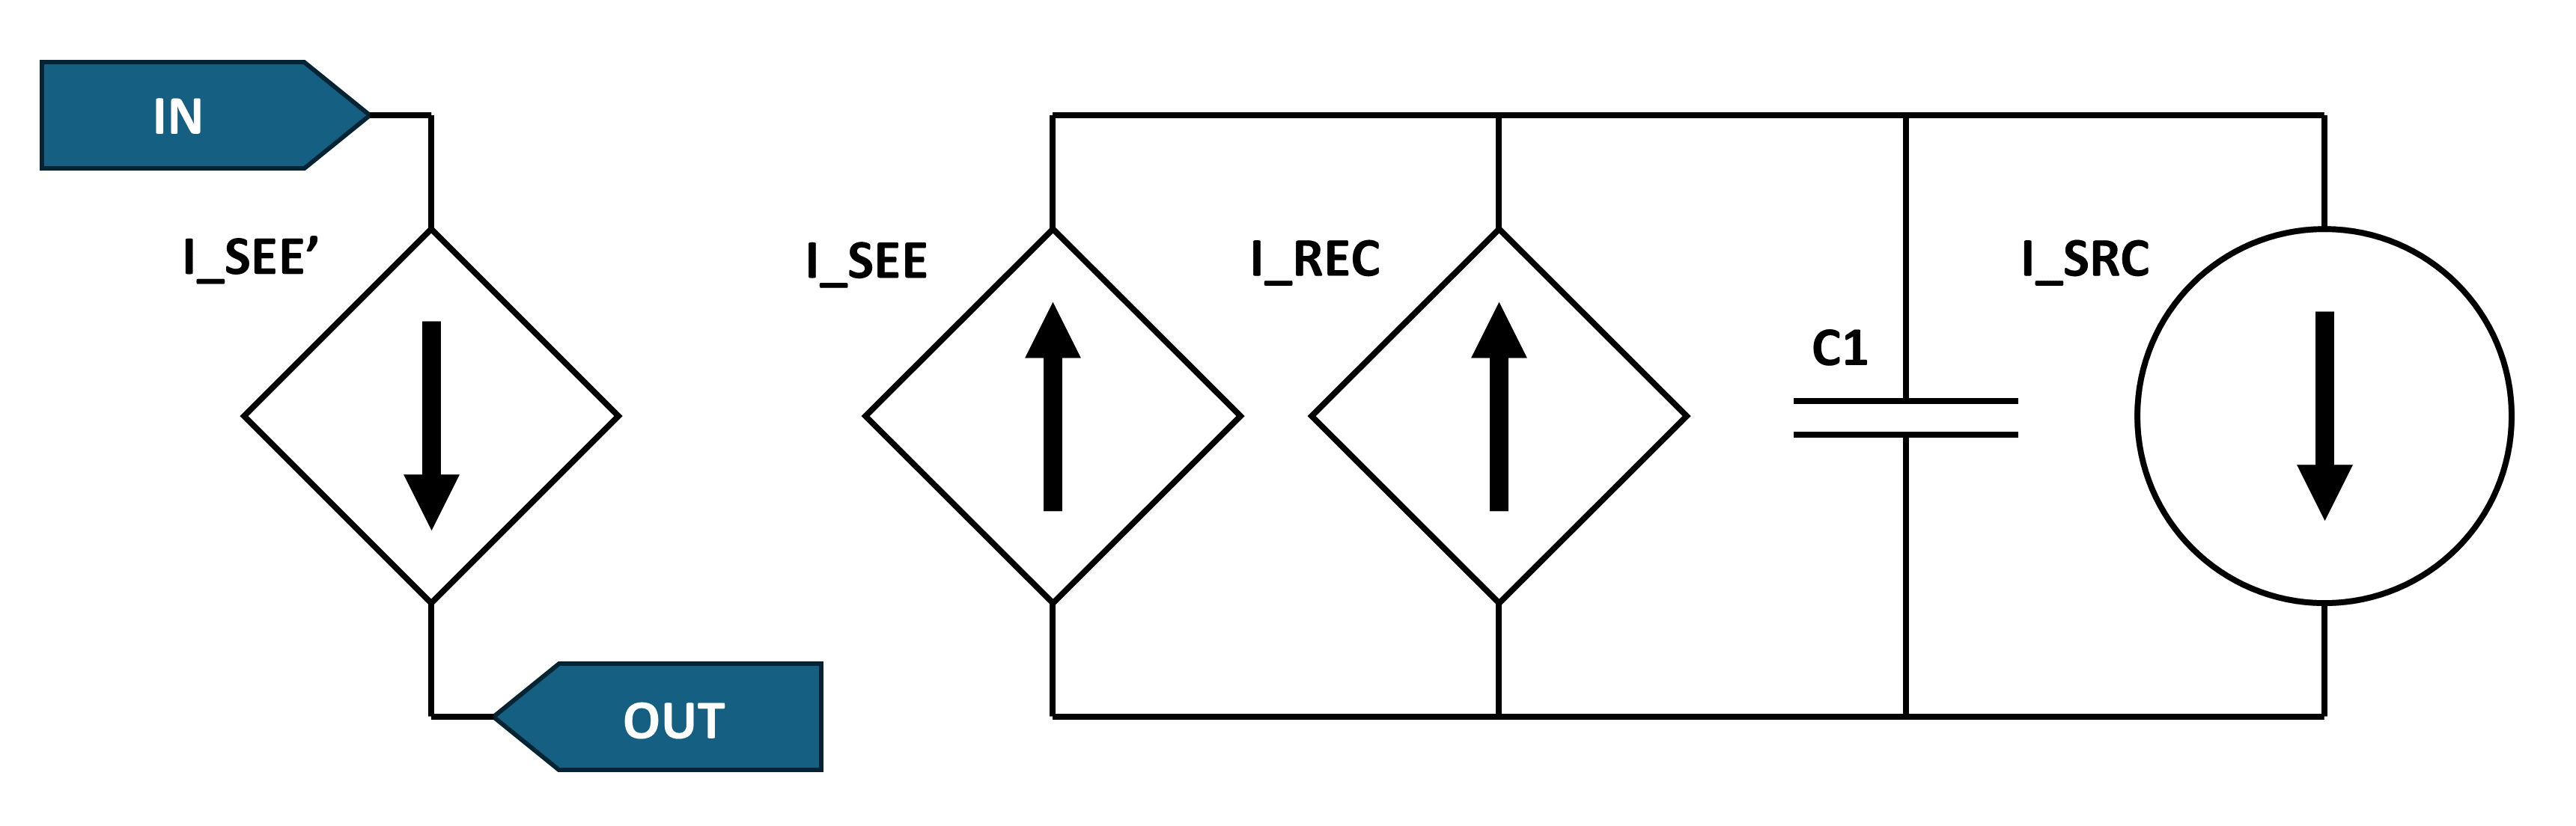
\includegraphics[width=0.95\linewidth]{Adaptive_Model_Cropped}
        \caption{Overview of adaptive double exponential current source model \cite{Kauppila2009}}
        \label{fig:adaptive_model_overview}
    \end{figure}

    The following equations define the behavior of the adaptive model:
            {\large
    \[B_{SEE}=Q(C1)*(V(IN)-V(OUT))*k\]
    }
    \(B_{SEE}\) (The observed current due to single event effects) is a function of the total charge stored in the capacitor, the voltage across the adaptive current source, and an adjustment constant \(k\).
            {\large
    \[B_{REC}=recomb\_adj*Q(C1)*k\]
    }
    \(B_{REC}\) (The current due to electron-hole pair recombination effects) is a function of an adjustment parameter \(recomb\_adj\), the total charge on the capacitor, and a second adjustment constant \(k\).
    Note, this \(k\) is the same \(k\) as presented in the equation for \(B_{SEE}\).
            {\large
    \[B_{SEE}'=I(B_{SEE})\]
    }
    \(B_{SEE}'\) is a current mirror of \(B_{SEE}\).
    This allows for the calculation portion of the circuit to be separated from outside influence.

    Lastly, \(I_{SRC}\) Is the standard double exponential current source built into most versions of SPICE\@.

    A description of each parameter in the adaptive current source is as follows:

    \begin{itemize}

        \item[] \(t_r\) - The simulation time at which charge injection begins

        \item[] \(t_f\) - The simulation time at which charge injection halts

        \item[] \(\tau_r\) - The rise time constant of \(I_{SRC}\)

        \item[] \(\tau_f\) - The fall time constant of \(I_{SRC}\)

        \item[] \(q_{tot}\) - The total charge to be injected into the node

        \item[] \(k\) - A constant for proportionally adjusting the drive strength of \(B_{SEE}\) and \(B_{REC}\)

        \item[] \(recomb\_adj\) - A constant for proportionally adjusting the drive strength of \(B_{REC}\)

    \end{itemize}
    \vspace{1em}

    \subsubsection{Usage}
    To simulate a single event effect on a PMOS transistor, a single event effect simulation block must be placed with the input of the block connected to the body node of the PMOS transistor and the output of the block connected to the drain node of the PMOS transistor.

    To simulate a single event effect on an NMOS transistor, a single event effect simulation block must be placed with the input of the block connected to the drain node of the NMOS transistor and the output of the block connected to the body node of the NMOS transistor. 
    Both of these configurations are demonstrated in figure~\ref{fig:SEE_Usage}. The reason behind these configuration restraints is beyong the scope of this paper.

    \begin{figure}[htbp]
        \centering
        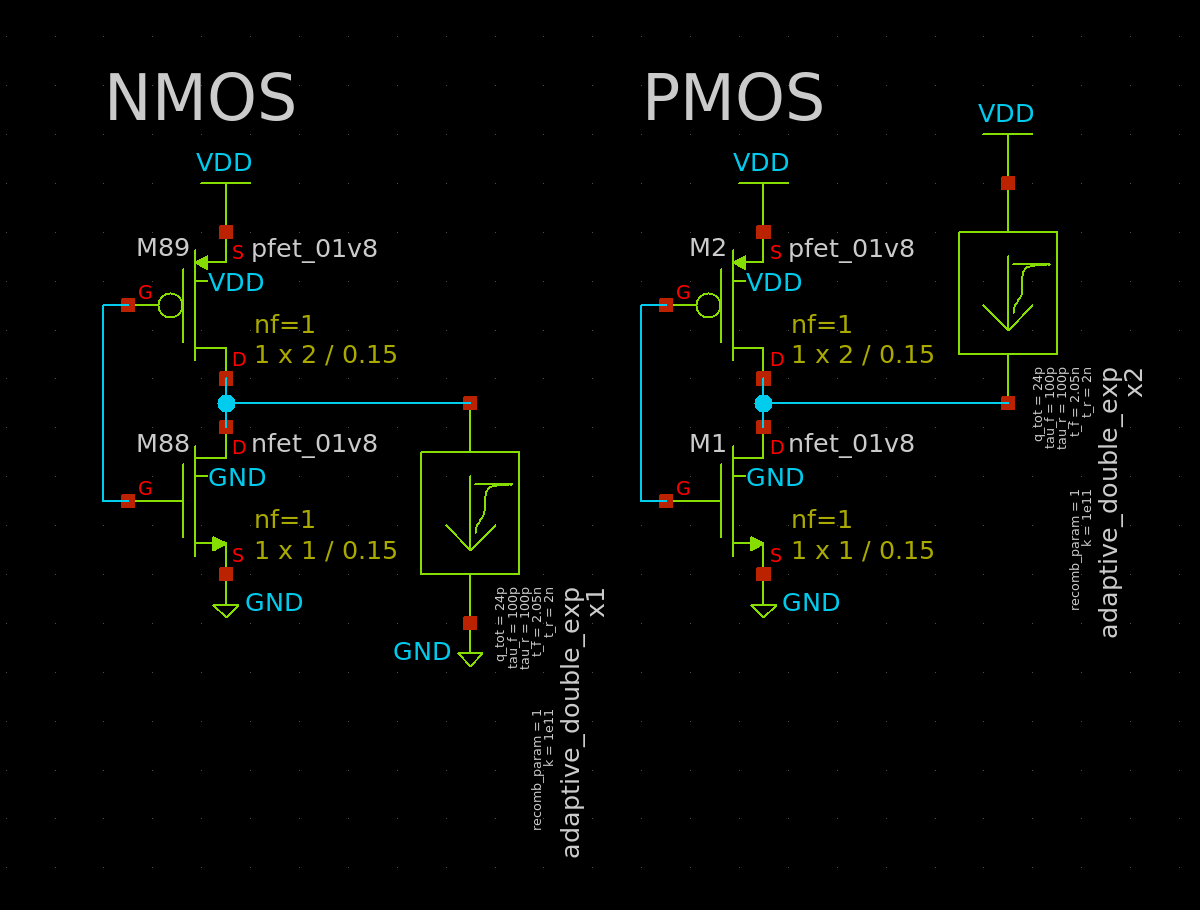
\includegraphics[width=0.9\linewidth]{PMOS_NMOS_Usage}
        \caption{Usage of SEE simulation modules on PMOS and NMOS transistors}
        \label{fig:SEE_Usage}
    \end{figure}


    \subsection{Other Radiation Effect Simulation}
    \label{subsec:other-radiation-effect-simulation}

    \subsubsection{TID Modules}
    TID, or total ionizing dose, is a radiation effect in which charge accumulates in the insulating regions of a MOSFET. This accumulation of charge can cause a number of undesirable affects.
    Some of the major affects that occur are a change in the threshold voltage of the MOSFET, and an increase in leakage current.
    We've chosen only to model the change in threshold voltage for the purposes of this paper.

    TID effects on MOSFET transistors cause the absolute value of the threshold voltage to decrease. This means that less voltage differential needs to exist between the gate and the source of the transistor to cause the transistor to transistion out of the cutoff region.

    We've chosen to model these effects as an inline voltage source that introduces a voltage bias into the signal driving the gate of the transistors.
    This, in effect, changes the threshold voltage for the MOSFET.
    [ADD CITATION]

    \vspace{1em}

    \subsubsection{Rail Span Collapse Voltage Source}
    A radiation induced phenomenon known as rail span collapse is often observed in complex circuits.
    Rail span collapse is characterized by the voltage between the positive and negative voltage rail collapsing due to excess current draw.
    This voltage collapse can result in severe problems, especially in circuity with sequential logic.

    One example where rail span collapse can cause issues is in an SRAM circuit.
    When an SRAM is irradiated, each time a reverse biased mosfet is struck a photo-current is generated in the junction.
    These photo-currents can be compounded together which can result in more current being drawn than the voltage rails can supply.
    This reduction in voltage difference between the positive and negative power rails can then cause the SRAM to become more susceptible to upsets, or lose its saved state all together.

    We've chosen to model voltage drop due to excessive current draw as a logistic function.
    This logistic function outputs a voltage drop for a given current draw as input.
    Figure \ref{fig:rail_collapse_function} shows an example plot of this model.

    \begin{figure}[htbp]
        \centering
        \includegraphics[width=0.95\linewidth]{rail_collapse_function}
        \caption{Rail span collapse function.}
        \label{fig:rail_collapse_function}
    \end{figure}

    In image \ref{fig:rail_collapse_function} the function is tuned such that significant voltage drop begins to occur once a current of 3mA is exceeded.
    When more than about 5mA is drawn the voltage source can no longer sustain the load and the voltage drop is near 1.8 volts.
    Given that the voltage source in this example has a nominal voltage of 1.8 volts, this means that there is near zero voltage between the positive and negative rails after 5mA\@.

    The following equations define the behavior of the rail span collapse model:
            {\Large
    \[V(I)=V_{nominal}-\frac{V_{nominal}}{1+e^{-k(I-I_0)}}\]
    }
    Where \(I_0\), the inflection point of the logistic function, is defined as:
            {\Large
    \[I_0=I_{limit}-\frac{\ln\left(\frac{V_{limit}}{V_{initial}-V_{limit}}\right)}{k}\]
    }

    A detailed description of each parameter in the rail span collapse voltage source is as follows:

    \begin{itemize}

        \item[] \(V_{nominal}\) - The nominal voltage of the voltage source under normal conditions

        \item[] \(V_{limit}\) - The voltage drop when a current of exactly \(I_{limit}\) is being drawn.
        Must be greater than zero

        \item[] \(I_{limit}\) - The maximum current draw before voltage drop occurs

        \item[] \(k\) - A constant for adjusting the slope of the logistic function

    \end{itemize}




    \section{Testing, Results, and Discussion}\label{sec:testing-results-and-discussion}
    This section presents the results of preliminary tests, highlighting the system's ability to simulate radiation effects with accuracy.
    
    Figure \ref{fig:inverter_response} depicts the voltage response of a CMOS inverter to a simulated radiation strike generated by the adaptive double exponential current source on the reverse biased NMOS transistor. The waveform generated closely resembles results found from TCAD simulations. \cite{Kauppila2009}
    
        \begin{figure}[htbp]
        \centering
        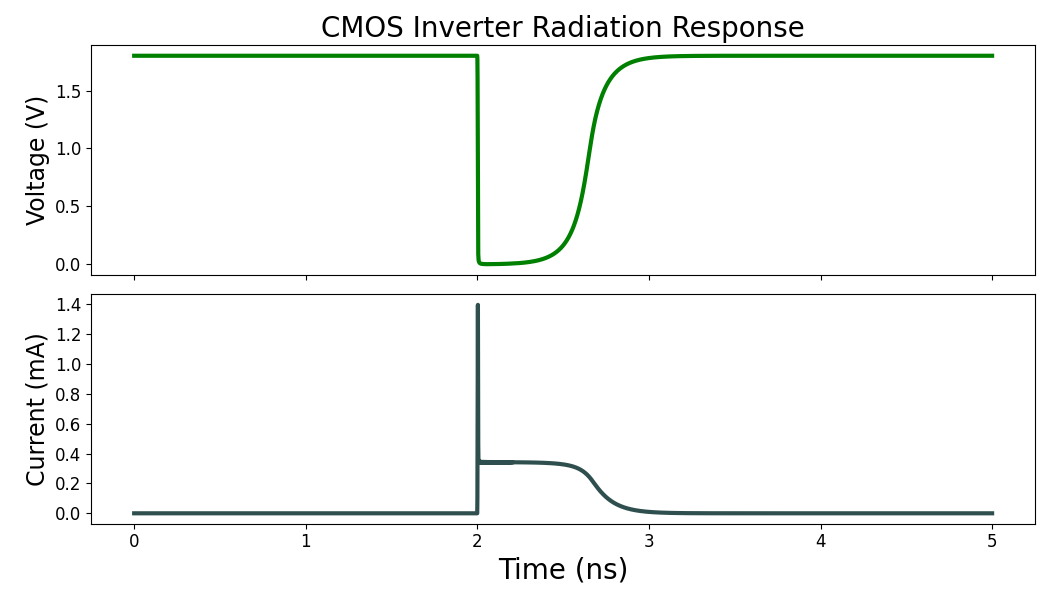
\includegraphics[width=0.95\linewidth]{Inverter_Response}
        \caption{Voltage response of CMOS inverter due to simulated radiation strike on NMOS transistor}
        \label{fig:inverter_response}
    \end{figure}
    
Figure \ref{fig:rail_collapse_response} depicts the voltage response of the rail span collapse voltage source to an arbitrary current draw. In this example, the threshold current before rail collapse begins is set at 8.7 mA.

    \begin{figure}[htbp]
        \centering
        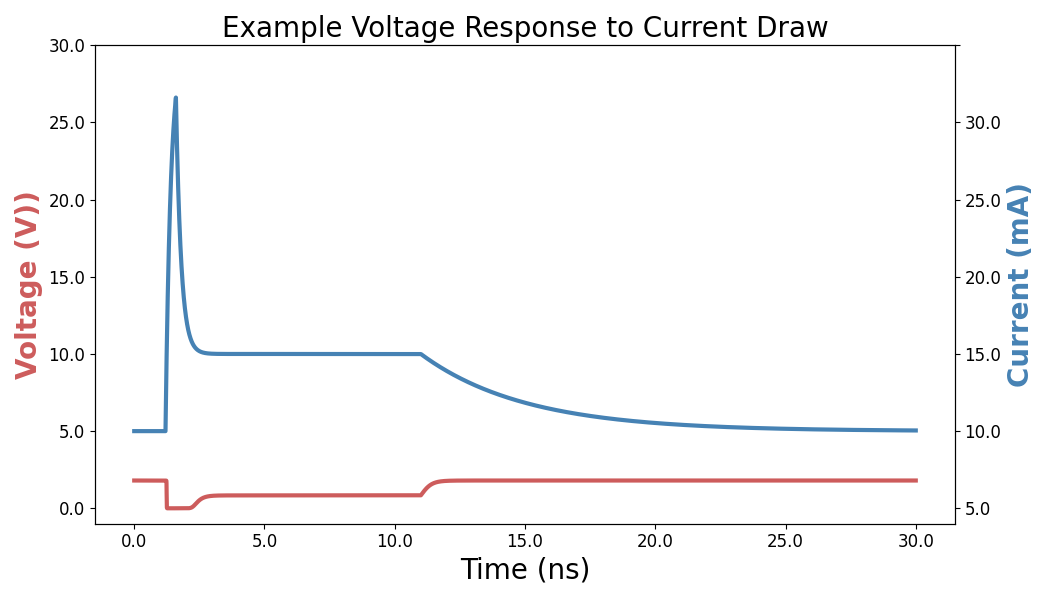
\includegraphics[width=0.95\linewidth]{Rail_Collapse_Response}
        \caption{Voltage output in response to excess current draw.}
        \label{fig:rail_collapse_response}
    \end{figure}~\cite{Massengill1984}.


    %\subsection{Generalization and Application}\label{subsec:generalization-and-application}
    %This subsection explores the potential for generalizing the simulation method to other types of circuits and its applicability in various fields requiring precise radiation effect simulation~\cite{Pepper1990}.


    \section{Conclusion and Future Work}\label{sec:conclusion-and-future-work}
    This paper presented an open-source radiation hardening simulator designed to simulate and analyze the effects of radiation on electronic circuits.
    The simulator integrates Xschem and NGSpice with custom-developed modules for fault injection, and radiation effect simulation.
    The incorporation of advanced models for Single Event Effects (SEE) and Total Ionizing Dose (TID) has shown accuracy in preliminary tests, demonstrating the system's potential for reliable simulations.

    In future work, we plan to further optimize the simulator and explore additional features.
    We aim to enhance the simulator's capability to handle more complex scenarios and to improve its user interface for better usability.
    Additionally, we will investigate potential collaborations with other research projects to expand the simulator's applications and impact~\cite{Pepper1990}.
    Future developments will focus on refining the adaptive models and integrating more comprehensive radiation effect simulations to support a wider range of research and practical applications.

    \section*{Acknowledgment}
    The authors would like to thank Dr. Shiuh-hua Wood Chiang for his guidance and support throughout this project.
    We also acknowledge the contributions of our colleagues and the funding support from [Funding Source].
    Their assistance has been invaluable in the development and success of this project.

    \bibliographystyle{IEEEtran}
    \bibliography{references}

\end{document}
